\chapter{An Example of Mathematical Writing}
\index{An Example of Mathematical Writing%
@\emph{An Example of Mathematical Writing}}%

\section{GreenWeb: Web Language Extensions for Energy-Efficient Web Computing}
\label{sec:lang}

%Web application developers today must be conscious of energy efficiency. Current abstractions between software and hardware, however, do not provide developers opportunities to optimize for energy efficiency. Instead, energy optimizations are mostly conducted at the hardware and OS level via techniques such as dynamic voltage and frequency scaling. Although effective from a hardware perspective, the key limitation of these techniques is that they are not aware of user quality-of-service (QoS) expectation and may lead to poor experience~\cite{big-little, ebs, pgdvfs}. Failing to deliver desirable QoS experience can cause severe consequences. For example, a 1-second delay in webpage load time costs Amazon \$1.6 billion annual lost in sales~\cite{Eaton:2013uq}.

Web languages are at the interface between applications and Web runtime. Traditionally, Web developers use Web languages to express structure, style, and functionality of an application while relying on the underlying system to perform energy optimizations without compromising user QoS experience. However, without being informed with the QoS information, the runtime system might not always effectively reason about the trade-off between QoS and energy consumption.

To better guide runtime optimizations, I present \greenweb, a set of Web language extensions that allow Web developers to express user QoS expectation at an abstract level. Based on the programmer-guided QoS information, the runtime substrate of \greenweb could then dynamically determine how to deliver the target QoS experience while minimizing the energy consumption.

%To help Web developers easily express QoS information in Web applications, our \textit{key insight} is that user QoS experience can be sufficiently captured by two fundamental abstractions: \textit{QoS type} and \textit{QoS target}. Intuitively, QoS type characterizes whether users perceive QoS experience by ``interaction responsiveness'' or ``animation smoothness'', and QoS target denotes the performance level that is required to deliver a desirable user experience for a specific QoS type. \greenweb provides specific language constructs for expressing the two QoS abstractions and thus empowering Web developers to provide ``hints'' to guide energy optimizations.

In this section, I first discuss the relationship between QoS, performance, and energy consumption. It lays the foundation of abstracting user QoS experience~(\Sect{sec:lang:eqos}). I then introduce QoS type and QoS target as two fundamental abstractions that capture two critical aspects of user QoS experience~(\Sect{sec:lang:abst}). I then present the design and specification of \greenweb, a group of Web language extensions that allows developers to easily express the two QoS abstractions~(\Sect{sec:lang:spec}). I further discuss the relationship between the \greenweb extensions and the \webrt runtime~(\Sect{sec:lang:inter}), and argue that \greenweb and \webrt are synergistic while independent. Finally, I discuss \greenweb in the general context of language support for performance and energy-efficiency~(\Sect{sec:lang:related}).

\subsection{Trade-off Between QoS, Performance, and Energy}
\label{sec:lang:eqos}

We illustrate the relationship between application QoS, performance, and energy savings in~\Fig{fig:eqos}. Performance degrades from left to right on the~\textit{x}-axis. The left and right~\textit{y}-axes indicate QoS and energy savings, respectively. Foundational work in human-computer interaction research~\cite{eventlatency, designUI, info_vis, response_time, percent_done, usability_engineering} indicates that interactive application QoS can be classified into three distinct states as machine performance degrades: \textit{imperceptible} $[P_H,P_I]$, \textit{tolerable} $(P_I,P_U]$, and \textit{unusable} $(P_U,P_L]$.

\begin{figure}[h]
\centering
\captionsetup{width=.7\columnwidth}
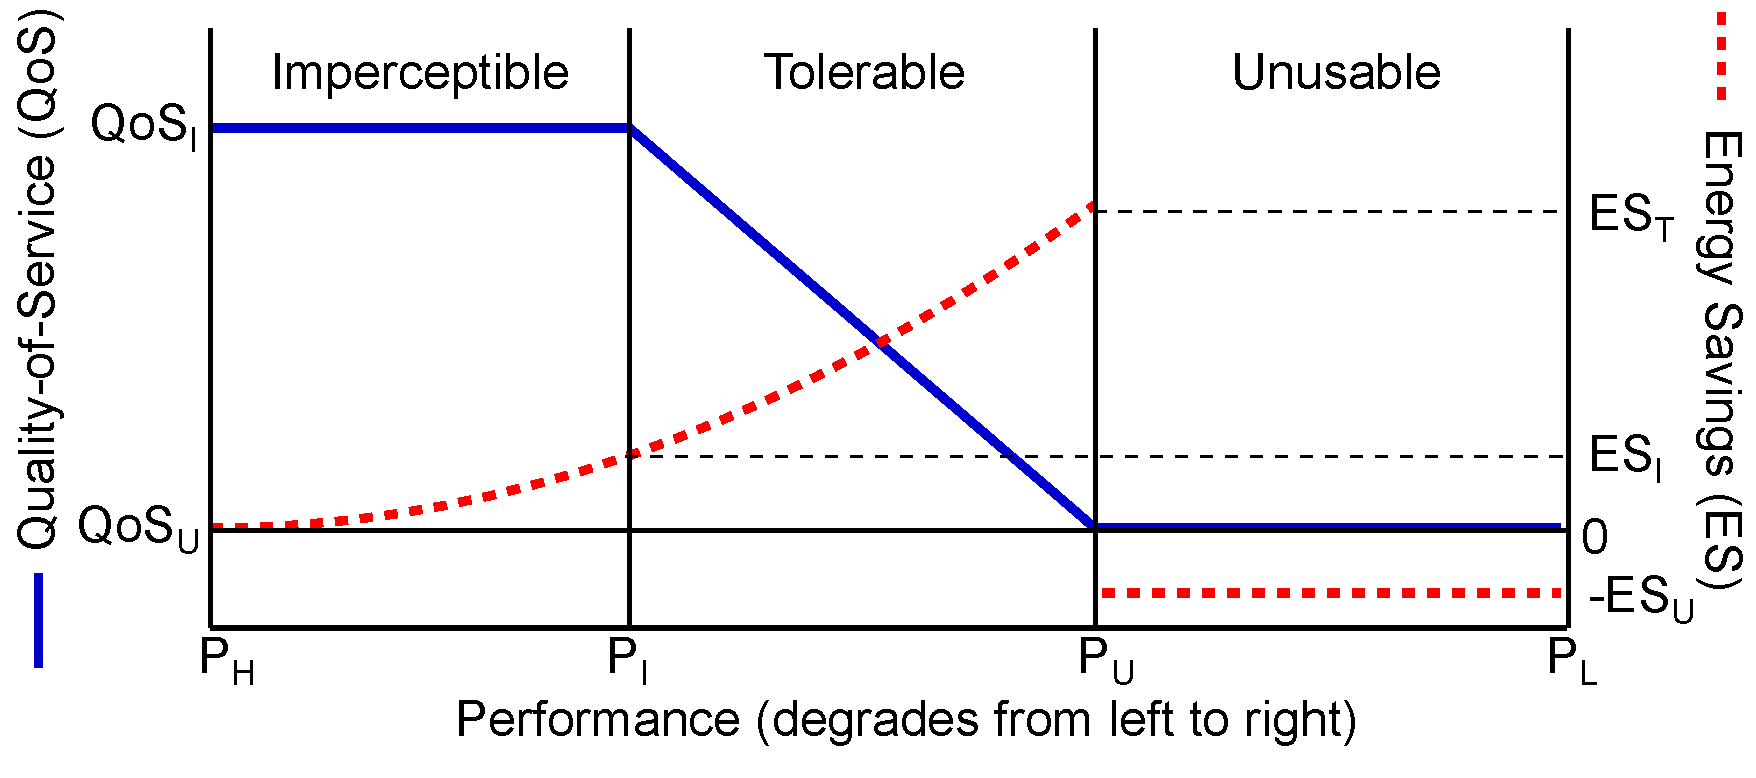
\includegraphics[trim=0 0 0 0, clip, width=.6\columnwidth]{eqos}
\caption{\small{The interplay between QoS, performance, and energy.}}
\label{fig:eqos}
\end{figure}

In the imperceptible region, performance can degrade without any user-perceptible QoS loss while achieving more energy savings. Imperceptible QoS, $QoS_I$, is maintained until performance reaches $P_I$, the lowest performance level that provides $QoS_I$. In the imperceptible region, supplying higher performance simply leads to more energy waste without adding any end-user value. For example, the most conservative approach to guarantee application QoS is to supply the peak performance of $P_H$; it leads to an energy waste of $ES_I$. Beyond $P_I$, application QoS enters the tolerable region, where QoS deteriorates as performance reduces, but still remains tolerable. Any QoS could be acceptable in this region depending on the usage scenario or specific user pattern~\cite{usagepattern, satscore}. Therefore, the tolerable QoS region exhibits a traditional performance-energy trade-off space. As performance further degrades, QoS is eventually violated at $P_U$, which is the performance limit where users no longer feel engaged by the application. At $P_U$ and beyond, users abandon the service. As a result, any energy consumed up until the service abandonment ($ES_U$) is wasted, because the underlying computation does not provide any utility to the user.

In summary, QoS-aware energy-efficiency optimization implies one of the following two optimization strategies depending on user QoS expectation. First, when the QoS expectation is high, guarantee imperceptible QoS experience with the minimal energy by exploiting the performance slack between $P_H$ and $P_I$. Second, when the user QoS expectation is low, guarantee usable QoS experience with the minimal energy by achieving a performance of $P_U$.

\subsection{QoS Abstractions for Web Applications}
\label{sec:lang:abst}

Abstracting user QoS experience is the prerequisite in expressing QoS information in a programming language. Based on the understanding of the interplay between QoS and energy consumption, I propose the QoS type and QoS target abstractions. I discuss why they are necessary and sufficient to capture user QoS experience for QoS-aware energy-efficiency optimizations.

\paragraph{QoS Type} We define an abstraction called \textit{QoS type} to capture different ways that users interpret QoS experience. Two major QoS types exist: \textit{single} and \textit{continuous}. Intuitively, they indicate whether the QoS experience is determined by the ``responsiveness'' of a single frame or the ``smoothness'' of a continuous sequence of frames, respectively. Alternatively, one can think of QoS type as the metric of concretizing performance ($x$-axis) in \Fig{fig:eqos}.

\begin{itemize}
\item Some user interactions produce only a single frame, which we call the response frame. The QoS type of these interactions is ``single,'' indicating that user QoS experience is determined by the latency at which the response frame is perceived by users~\cite{eventlatency}. For instance, imagine a fingertap interaction that opens a search box in a Web application. Users perceive the effect of the fingertap when the application displays a response frame---the frame with the search box displayed. Web application loading process also falls in this category. This is because although there are several intermediate frames being produced during the loading process, user QoS experience is largely determined by the latency to deliver the ``first meaningful frame''~\cite{fmf}, which indicates that a Web application is usable to users.

\item The other QoS type is ``continuous,'' corresponding to interactions whose responses are not one single frame but a sequence of continuous frames. User QoS experience is determined by the latency of \textit{each} frame in the sequence, rather than one particular frame.

Continuous frames are often found in the form of animations. The simplest form of animation is triggered by finger moving such as scrolling. Tapping can also cause a sequence of frames to be generated. For instance, many Web applications provide a navigation button that dynamically expands when tapped and generates an animation. More complex animations in Web applications can be controlled by \texttt{requestAnimationFrame} (\texttt{rAF}) APIs~\cite{animationtiming} and CSS animation/transition~\cite{cssanimations, csstransitions}.
\end{itemize}

QoS type is an important abstraction because optimizing for a wrong QoS type may lead to energy-inefficient decisions. For example, imagine a fingtertap that only produces one frame  (e.g., displaying a search box). A Web runtime that mistakenly optimizes for ``continuous'' frame latency may force the hardware to run at its peak performance in order to produce frames even when no frame is intended, leading to energy waste. ``Single'' and ``continuous'' are two unique QoS types that must be differentiated.


\begin{table}[t]
\Huge
\centering
\captionsetup{width=.6\columnwidth}
\caption{\small Mobile Web interactions fall into three categories based on different QoS type and QoS target combinations.}
\renewcommand*{\arraystretch}{1.2}
\renewcommand*{\tabcolsep}{12pt}
\resizebox{.6\columnwidth}{!}
{
  \begin{tabular}{l l l}
  \toprule[0.15em]
  \bigstrut\textbf{QoS Type} & \bigstrut\textbf{\specialcell{QoS Target\\($P_I$, $P_U$)}} & \multicolumn{1}{c}{\bigstrut\textbf{~~~~~~~~~~~Description}}\\
  \midrule[0.05em]
  Continuous & (16.6, 33.3) ms & \specialcell{QoS experience is evaluated\\by \textit{continuous} frame latencies.} \\
  \midrule
  \multirow{2}{*}[-33pt]{Single} & (100, 200) ms & \specialcell{QoS experience is evaluated by
\\a \textit{single} frame latency. Users
\\expect \textit{short} response period.} \\
  & (1, 10) s & \specialcell{QoS experience is evaluated by
\\a \textit{single} frame latency. Users
\\expect \textit{long} response period.} \\
  \bottomrule[0.15em]
  \end{tabular}
}
\label{tab:qos_info}
\end{table}

\paragraph{QoS Target} Another critical QoS abstraction is \textit{QoS target}, denoting the performance level needed to deliver a certain QoS experience. Two different QoS targets exist that are critical to user experience: imperceptible target ($P_I$) and usable target ($P_U$)~\cite{ebs}. They correspond to the imperceptible and usable QoS experience discussed in \Fig{fig:eqos}. We use frame latency as a natural choice for the performance metric because frame updates dictate QoS experience. Specifically, we define frame latency as the delay from when an event is initiated by a user to when its corresponding frame(s) show on the display.

\begin{itemize}
\item For interactions with a ``single'' QoS type, QoS target depends on the complexity of the interaction~\cite{eventlatency}. For interactions that are expected to finish quickly, user latency tolerance is low. For instance, a fingertap that displays a search box falls into this category because displaying a search box is inherently expected to finish ``instantly.'' For these ``lightweight'' interactions, users feel the system is responding instantly at 100~ms, and start thinking that the system is not working after 300~ms~\cite{humanperception}. Thus, 100~ms and 300~ms can be used as the $P_I$ and $P_U$ values, respectively.

In contrast, when users are aware of a computationally intensive job being processed, they tend to have high tolerance for latencies~\cite{usability_engineering}. Psychology studies show that users can subconsciously wait up to 1 second for a job to complete while still staying focused on the current train of thought. Once a job execution exceeds 10 seconds, user attentions are distracted and cannot tolerate the delay~\cite{info_vis, response_time}. Therefore, 1 second and 10 seconds can be treated as the $P_I$ and $P_U$ values for ``heavyweight'' interactions, respectively.

\item For interactions with a ``continuous'' QoS type, 60 and 30 frames per second (FPS) deliver a ``seamless'' and ``just playable'' user experience, respectively~\cite{fps_target}. Thus, a performance level that guarantees 16.6~ms and 33.3~ms frame latency can be regarded as the imperceptible and usable QoS target, respectively. It is worth noting that the QoS target applies to each frame rather than an average latency. This is because human eyes are very sensitive to frame variance. Tiny hitches in a high volume of frames can cause a poor QoS experience and even headaches~\cite{jankbusting, adaptivevsync}.
\end{itemize}

User interactions fall into three distinct categories based on different QoS type and QoS target combinations as listed in \Tbl{tab:qos_info}. Although the absolute values of QoS target ($P_I$ and $P_U$) in each category can vary slightly with user perceptibility, their magnitudes differ significantly across categories (i.e., tens of milliseconds versus hundreds of milliseconds versus seconds). Thus, QoS target is an important abstraction to differentiate different performance requirements.

\subsection{QoS-Aware Web API Design}
\label{sec:lang:spec}

%\begin{figure}[t]
%  \centering
%  \captionsetup{width=.6\columnwidth}
%  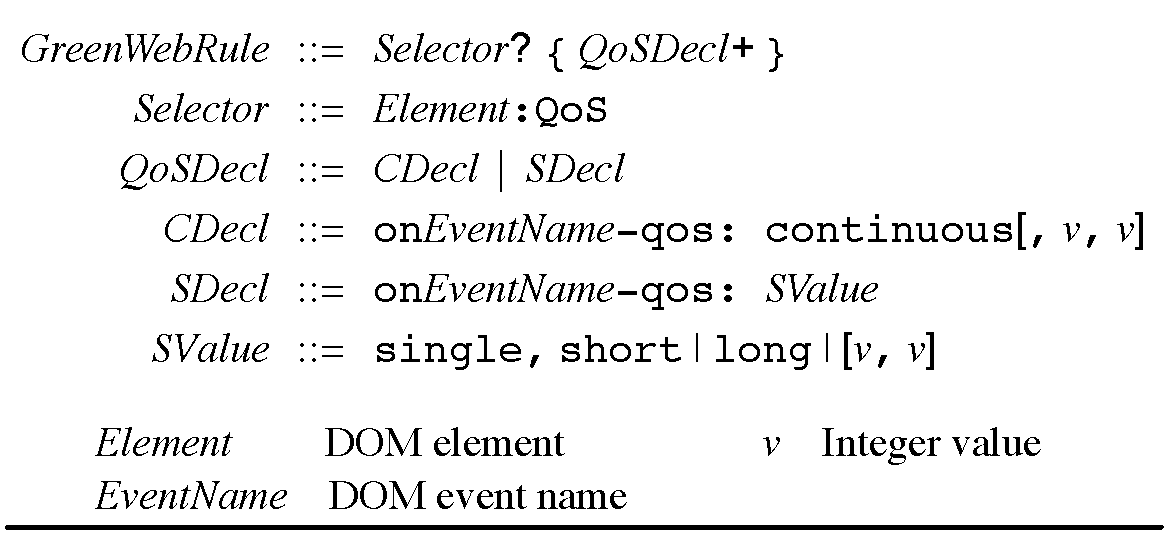
\includegraphics[trim=0 0 0 0, clip, width=.6\columnwidth]{syntax}
%  \caption{\small{The syntax of \greenweb language extensions.}}
%  \label{fig:syntax}
%\end{figure}
%CSS syntax for reference
%http://www.w3.org/TR/2003/WD-css3-syntax-20030813/
%http://www.w3.org/TR/CSS21/grammar.html
%https://developer.mozilla.org/en-US/docs/Web/CSS/Value_definition_syntax

We present \greenweb, a set of Web language extensions that lets application developers easily express the two QoS abstractions as program annotations. \greenweb APIs extend current CSS language to specify QoS type and QoS target information. We choose CSS because its syntax and semantics naturally allow us to select DOM elements and specify various characteristics. The core of CSS is a set of \textit{style rules} \cite{css21}. Each style rule selects specific Web application elements and sets their style properties. A style rule expresses such semantics through two language constructs: a \textit{selector}, which selects specific Web application elements, and a set of style \textit{declarations}, which are $\langle property, value \rangle$ pairs that assign $value$ to $property$. As an example, the following CSS rule \texttt{h1 \{font-weight: bold\}} selects all the \texttt{h1} elements and sets their \texttt{font-weight} property to \texttt{bold}.

%Traditionally, CSS supports only pure visual style properties such as fonts and colors. Recent development of CSS languages (e.g., CSS3~\cite{mdncss3}) lets developers express richer information such as controlling animations~\cite{cssanimations} and adapting to different device form factors~\cite{css3mediaquery}. \greenweb follows such a spirit of CSS language evolution and expands its scope to allow expression of use QoS experience related information.

\Tbl{tab:api_spec} lists semantics of each \greenweb API. Intuitively, each \greenweb API selects an application element \texttt{E}, and declares CSS properties to express the QoS type and QoS target information when an event \texttt{onevent} is triggered on \texttt{E}. We now describe the details of \greenweb extensions.

\begin{table}[t]
\Huge
\centering
\captionsetup{width=.7\columnwidth}
\caption{\small \greenweb API specification. Each API is a CSS rule specifying the QoS information when a particular event is triggered on a Web element.}
\renewcommand*{\arraystretch}{1.1}
\renewcommand*{\tabcolsep}{8pt}
\resizebox{.7\columnwidth}{!}
{
    \begin{tabular}{l l}
    \toprule[0.15em]
    \bigstrut\textbf{Syntax} & \bigstrut\textbf{Semantics} \\
    \midrule[0.05em]
    \specialcell{\texttt{\textcolor{blue}{E:QoS} \{}
\\~~~~\texttt{\textcolor{Green}{onevent-qos:} continuous;}
\\\texttt{\}}} & \specialcell{As soon as \texttt{onevent} is triggered on\\DOM element \texttt{E}, the application must\\continuously optimize for frame latency.\\Use the $P_I$ and $P_U$ values in \Tbl{tab:qos_info} as\\the default QoS target for all frames.}\\
    \midrule[0.05em]
    \specialcell{\texttt{\textcolor{blue}{E:QoS} \{}
\\~~~~\texttt{\textcolor{Green}{onevent-qos:} single,}
\\~~~~\texttt{~~~~~~~~~~~~~~short|}
\\~~~~\texttt{~~~~~~~~~~~~~~~long}
\\\texttt{\}}} & \specialcell{Once \texttt{onevent} is triggered on element\\\texttt{E}, the application must optimize for the\\latency of the single frame caused by\\ \texttt{onevent}. Users expext short (longer)\\latency. Use the $P_I$ and $P_U$ values in\\\Tbl{tab:qos_info} as the default QoS target.}\\
    \midrule[0.05em]
    \specialcell{\texttt{\textcolor{blue}{E:QoS} \{}
\\~~~~\texttt{\textcolor{Green}{onevent-qos:} continuous|}
\\~~~~\texttt{~~~~~~~~~~~~~~~~~single,}
\\~~~~\texttt{~~~~~~~~~~~~~~~ti-value,}
\\~~~~\texttt{~~~~~~~~~~~~~~~tu-value,}

\\\texttt{\}}} & \specialcell{Explicitly specify $P_I$ (\texttt{ti-value}) and\\$P_U$ values (\texttt{tu-value}) for QoS targets.\\Note that both values must either appear\\or be ommitted together.}\\
    \bottomrule[0.15em]
    \end{tabular}
}
\label{tab:api_spec}
\end{table}

\paragraph{Selector} To decorate a CSS rule as specifying QoS information of an element, we define a new CSS pseudo-class selector~\cite{css_pseudo_class} ``\texttt{:QoS}.'' An element \texttt{E} is selected using existing selectors, such as ID (\texttt{\#id}) and Class (\texttt{.class}) selectors, before applying the \texttt{:QoS} pseudo-class qualifier. For example, \texttt{div\#intro:QoS} selects the \texttt{div} element with the ID \texttt{intro} before declaring QoS information.

\paragraph{Property} QoS information is expressed as CSS properties in \greenweb. We define a new CSS property called \texttt{onevent-qos}, in which \texttt{onevent} is a DOM event that \greenweb supports. In its simplest form, \texttt{onevent-qos} could be set to \texttt{continuous} (first rule in \Tbl{tab:api_spec}). The semantics of declaring \texttt{onevent-qos: continuous} is that as soon as \texttt{onevent} is triggered on element \texttt{E}, the runtime must continuously optimize for frame latency until the last relevant frame is generated.

To express the ``single'' QoS type, the \texttt{onevent-qos} property accepts a list of two values separated by a comma, one to indicate that the QoS type is single, and the other to indicate whether users expect a short or long execution period (second rule in \Tbl{tab:api_spec}). For instance, the declaration \texttt{onevent-qos: single, short} expresses that the runtime must optimize for the latency of the single frame caused by \texttt{onevent}, and users expect short frame latency.

Developers do not have to specify the QoS target values, and the \greenweb runtime will use the $P_I$ and $P_U$ values in \Tbl{tab:qos_info} as the default QoS target. However, we also provide the flexibility for developers to overwrite default QoS targets. This is achieved by specifying absolute values of $P_I$ and $P_U$ (in milliseconds) after \texttt{single} or \texttt{continuous}, as illustrated by the third rule in \Tbl{tab:api_spec}.

\subsection{GreenWeb and WebRT Inteplay}
\label{sec:lang:inter}

Combing \greenweb and \webrt in an integrated system would provide programmers an opportunity to guide runtime energy-efficiency optimizations by providing QoS ``hints.'' This approach would be both \textit{precise} and \textit{efficient}. It is precise because only developers have the exact knowledge of code logic. They can provide QoS type and target information that is difficult for the runtime to infer. It is efficient because it does not entail performance and energy overhead of runtime detection. Such a design philosophy is similar to traditional pragma-based programming APIs such as OpenMP. For example, the ``\texttt{omp for}'' pragma in OpenMP indicates that iterations in a \texttt{for} loop are completely independent such that the runtime can safely parallelize the loop without the need to check for correctness. Similarly, \greenweb annotations would allow the Web runtime to perform ``best-effort'' optimizations without having to infer QoS information. I leave the full integration and evaluation of such a language-runtime co-designed system as future work.

It is worth noting that although \greenweb and \webrt are compatible and can be integrated, they by design are independent systems. \greenweb is independent of \webrt because it does not pose constraints on specific runtime implementations. It is possible to use the ACMP-based \webrt as a \greenweb runtime implementation to make QoS-energy trade-offs at the hardware level. It is also feasible to build a runtime leveraging only a single big (or little) core capable of DVFS~\cite{pgdvfs, vsmp}. In addition, one could implement a \greenweb runtime using pure software-level techniques, such as prioritizing resource loading~\cite{klotski} or using power-conserving colors~\cite{chameleon}. 

\webrt is also independent of \greenweb because it by design does not rely on programmer-assisted annotations to perform scheduling. Without QoS ``hints'' from the application, the \webrt schedulers can assume a default QoS target and QoS type for each Loading, Touching, and Moving interaction. The \webrt schedulers can also attempt to infer the QoS type and QoS target by profiling event executions to identify which category in \Tbl{tab:qos_info} that an event falls into. I leave the quantitative comparison between unguided and \greenweb-guided \webrt to future work.

\subsection{Related Work}
\label{sec:lang:related}

\paragraph{Language Support for Web Performance} The Web community has a long tradition of providing language extensions that allow developers to specify ``hints'' for browsers. The focus, however, has been primarily on \textit{performance} optimizations. \greenweb, to the best of our knowledge, is the first Web language extension that specifically targets \textit{energy}.

The most classical example of performance hint is link prefetch~\cite{linkprefetch}, which lets Web developers use an HTML tag to specify that a particular link will likely be fetched in the near future. With such information, a Web browser could prefetch the link when there are no on-demand network requests. Another example is the CSS \texttt{willChange} property~\cite{csswillchange}, which hints browsers about what visual changes to expect from an element so that the browser could perform a computationally intensive task ahead of time. Similar to \texttt{willChange}, \greenweb introduces a new CSS property \texttt{onevent-qos}, which allows providing QoS-related hints.

\paragraph{Language Support for Energy Efficiency} Language support for energy-efficiency has recently become an important research thrust. Most work targets approximate computing and sensor-based applications. To the best of our knowledge, this is the first work that focuses on Web applications. Green~\cite{green} provides APIs that let developers specify approximate versions of a function and QoS loss constraints. EnerJ~\cite{enerJ} takes the language support for approximate computing a step further by designing a general type system. These language frameworks could be applicable if sources of approximation in Web applications are identified, which however is beyond our scope. LAB~\cite{lab} identifies latency, accuracy, and battery as fundamental abstractions for improving energy-efficiency in sensor-based applications. Similarly, \greenweb identifies the QoS type and QoS target abstractions for enabling energy-efficient Web applications.
